% Tormenta: CT-378 Machine Learning final report, IEEE conference format (IEEEtran).
% Compile on Overleaf (pdfLaTeX) or with tectonic. Upload the whole docs/report/final/ folder; figures are in figs/.
% Graphs are drawn at column width by `python -m src.report_figures`; screenshots are of the live Streamlit app.
\documentclass[conference,a4paper]{IEEEtran}
\IEEEoverridecommandlockouts
\usepackage{cite}
\usepackage[T1]{fontenc}
\usepackage{newtxtext,newtxmath}   % Times, the IEEE body font
\usepackage{iftex}                 % sans serif for the cover page only: Helvetica (pdfLaTeX) or its clone (XeTeX)
\ifXeTeX
  \usepackage{fontspec}
  \setsansfont{texgyreheros}[Scale=0.92, Extension=.otf, UprightFont=*-regular, BoldFont=*-bold,
    ItalicFont=*-italic, BoldItalicFont=*-bolditalic]
  \newcommand{\coverfont}{\sffamily}
\else
  \usepackage[scaled=0.92]{helvet}
  \newcommand{\coverfont}{\fontfamily{phv}\selectfont}
\fi
\usepackage{amsmath}
\usepackage{graphicx}
\usepackage{booktabs}
\usepackage{array}
\usepackage{tabularx}
\usepackage{xcolor}
\usepackage{tikz}
\usetikzlibrary{arrows.meta,positioning}
\usepackage{placeins}
\usepackage{balance}               % balance the two columns on the last page
\usepackage{url}
\usepackage[hidelinks]{hyperref}
\graphicspath{{figs/}}
\renewcommand{\topfraction}{0.92}
\renewcommand{\bottomfraction}{0.8}
\renewcommand{\textfraction}{0.06}
\renewcommand{\floatpagefraction}{0.88}
\renewcommand{\dbltopfraction}{0.9}
\setcounter{topnumber}{4}
\setcounter{bottomnumber}{3}
\setcounter{totalnumber}{6}
\newcommand{\code}[1]{\texttt{\footnotesize #1}}
\newcolumntype{Y}{>{\raggedright\arraybackslash}X}

\title{Tormenta: Nowcasting and 7-Day Forecasting of Geomagnetic Activity with Machine Learning%
\thanks{CT-378 Machine Learning semester project, Fall 2026, submitted to Ms.\ Murk Marvi, Course Instructor.
Code: \url{https://github.com/Syeda-Aliza-Ayaz/Tormenta}; live app: \url{https://tormenta.streamlit.app/}.}}
\author{\IEEEauthorblockN{Syeda Aliza Ayaz}
\IEEEauthorblockA{Roll No.\ CT-24219\\
NED University of Engineering \& Technology\\
Karachi, Pakistan}
\and
\IEEEauthorblockN{Husn ur Rehman}
\IEEEauthorblockA{Roll No.\ CT-24070\\
NED University of Engineering \& Technology\\
Karachi, Pakistan}}

\definecolor{maroon}{HTML}{6B1F3A}
\definecolor{night}{HTML}{0B1426}
\definecolor{aurora}{HTML}{3DDC97}
\definecolor{ice}{HTML}{8EC5FF}
\definecolor{ink}{HTML}{1A2433}

\begin{document}

% ---------------------------------------------------------------- title page
\thispagestyle{empty}
% Cover page in the NED report style. Every element is placed absolutely, so it is always exactly one page.
\begin{tikzpicture}[remember picture, overlay]
  \def\W{14.6cm}
  \newcommand{\rulex}[1]{\draw[maroon, line width=0.9pt] ([xshift=-7.3cm, yshift=-#1]current page.north) -- ([xshift=7.3cm, yshift=-#1]current page.north);}
  \rulex{3.0cm}
  \node[font=\large, align=center] at ([yshift=-3.75cm]current page.north)
    {\textsc{NED University of Engineering \& Technology, Karachi}};
  \node[font=\small, align=center] at ([yshift=-4.3cm]current page.north)
    {Department of Computer Science \& Information Technology};
  \rulex{4.75cm}
  \node at ([yshift=-7.55cm]current page.north) {%
    \IfFileExists{figs/ned_logo.png}{
\includegraphics[height=4.6cm]{ned_logo.png}}%
    {\tikz\draw[gray, dashed] (0,0) circle (2.3cm) node[align=center, font=\small] {NED logo\\(figs/ned\_logo.png)};}};
  \node[font=\large, align=center] at ([yshift=-10.75cm]current page.north) {Machine Learning\\(CT-378)};
  \rulex{11.7cm}
  \node[font=\fontsize{22}{26}\selectfont\bfseries] at ([yshift=-12.6cm]current page.north) {Semester Project};
  \node[font=\Large] at ([yshift=-13.4cm]current page.north) {Project Report: TORMENTA};
  \node[font=\normalsize\itshape, align=center] at ([yshift=-14.05cm]current page.north)
    {Nowcasting and 7-Day Forecasting of Geomagnetic Activity with Machine Learning};
  \rulex{14.75cm}
  \node[anchor=north, font=\normalsize] at ([yshift=-15.6cm]current page.north) {%
    \renewcommand{\arraystretch}{1.15}%
    \begin{tabular}{@{}>{\bfseries}r@{\hspace{0.9em}}l@{}}
    Group Members: & Syeda Aliza Ayaz (CT-24219)\\
                   & Husn ur Rehman (CT-24070)\\
    Course:        & Machine Learning (CT-378)\\
    Instructor:    & Ms.\ Murk Marvi\\
    Assessment:    & Semester Project Report (with live demonstration)\\
    Technology:    & Python 3.12, scikit-learn, pandas, Streamlit, Flask, Hugging Face\\
    Live app:      & \url{https://tormenta.streamlit.app/}\\
    Code:          & \url{https://github.com/Syeda-Aliza-Ayaz/Tormenta}\\
    Submitted:     & November 2026\\
    \end{tabular}};
  \rulex{21.4cm}
  \node[font=\small, align=center] at ([yshift=-22.4cm]current page.north)
    {Bachelor of Science in Computer Science\\Academic Session 2024 -- 2028};
\end{tikzpicture}
\null
\clearpage

\maketitle

\begin{abstract}
Geomagnetic storms disturb power grids, satellites, GPS and HF radio; their strength is measured by the
planetary Kp index (0--9). Tormenta has two parts. The \textbf{nowcaster} estimates the current hour's Kp from
solar-wind measurements taken about an hour upstream of Earth: from 8 raw inputs we build 66 causal features, compare
a persistence baseline with Linear Regression, KNN, SVR, Random Forest and HistGradientBoosting tuned by 5-fold
time-ordered cross-validation, and reach a test RMSE of 0.573 Kp ($R^2$ 0.808, 34\% below persistence) with a
calibrated 80\% prediction interval. The \textbf{forecaster} predicts daily Ap and daily maximum Kp for the next
7 days, plus the probability of a storm day. Its final model adds daily solar wind and coronal-hole areas measured on
one solar image per day; on the 2020--2026 test period it beats an index-only model (skill 0.122 vs 0.100, gain
significant on days 2--5) and is level with NOAA's official forecast. Both are deployed on Streamlit Community
Cloud, the Hugging Face Hub and a local Flask app, and every forecast is logged and scored daily.
\end{abstract}

\begin{IEEEkeywords}
space weather, geomagnetic storms, Kp index, solar wind, gradient boosting, time-series forecasting, model deployment
\end{IEEEkeywords}

%=====================================================================================================================
\section{Problem and motivation}
The planetary \textbf{Kp index} summarises how strongly Earth's magnetic field is disturbed, one value per 3-hour
block on a 0--9 scale in thirds; \textbf{Ap} is its linear daily equivalent \cite{matzka2021}. Kp\,$\ge$\,5 is a
geomagnetic storm (NOAA scale G1 to G5). Storms induce currents in power grids, increase satellite drag, degrade GPS
and block HF radio. Official Kp is derived from ground magnetometers and published only after each block, with
final values weeks later.

Operators ask two different questions, and we answer both:
\begin{itemize}
\item \textbf{Nowcast: ``what is Kp right now?''} (regression, hourly). The solar wind that drives Kp is measured at
the L1 point, 1.5 million km upstream, about an hour before it reaches Earth. We estimate the current hour's Kp from
it alone; no geomagnetic index is an input, so the nowcast never waits for magnetometers.
\item \textbf{Forecast: ``how active will the next 7 days be?''} (regression + classification, daily). Daily Ap and
daily maximum Kp for lead days 1--7, and the probability of a storm day. Nobody measures the solar wind days ahead,
so the inputs are past activity, the 27-day solar rotation, the season, the solar wind now, and what is visible on
the Sun's Earth-facing side.
\end{itemize}
\textbf{Users:} grid and satellite operators, radio users and aurora watchers. \textbf{Success metrics:} RMSE on
held-out years against a baseline, storm-hour RMSE, coverage of the 80\% interval, and storm-warning skill compared
with NOAA SWPC's official forecasts \cite{swpc}.

%=====================================================================================================================
\section{Data collection}
We combine four public sources for the models and three more for benchmarks and experiments
(Table~\ref{tab:data}). All are downloaded by script, so the repository holds no raw data:
\code{python -m src.download\_data} rebuilds the core tables from nothing in about two minutes, and
\code{--all} adds the solar images and experiment datasets. Source, collection method, licence and access date of
every dataset are documented in \code{DATA.md}. None contains personal data.
\begin{itemize}
\item \textbf{Labels} are GFZ Kp; only values flagged \emph{definitive} are used for training and scoring.
\item Each hour of solar wind is labelled with the Kp of the 3-hour block that contains it, so the nowcaster's
245{,}688 hourly rows hold about 81{,}900 independent labels.
\item \textbf{NOAA's forecasts are a benchmark only}, never an input, so any skill we report is our own.
\end{itemize}

\begin{table*}[t]\centering\footnotesize
\caption{Datasets: content, collection method, licence, access date and size. Full details in \texttt{DATA.md}.}\label{tab:data}
\begin{tabularx}{\textwidth}{@{}p{2.6cm}Yp{4.1cm}p{2.3cm}p{1.6cm}p{1.9cm}@{}}\toprule
Dataset & Content & Collection method & Licence & Accessed & Size\\\midrule
\multicolumn{6}{@{}l}{\emph{Used by the models}}\\
NASA OMNI2 hourly \cite{king2005} & $|B|$, $B_x$, $B_y$, $B_z$ (GSM), speed, density, temperature at Earth's bow shock, 1998 $\to$ & NASA SPDF yearly files over HTTPS (\code{fetch\_omni.py}) & NASA public data & Oct--Nov 2026 & 245{,}688 hours\\
GFZ Potsdam Kp/Ap \cite{gfzkp} & 3-hourly Kp, ap; daily Ap; observed F10.7; definitive flag; 1932 $\to$ & HTTPS text file, refreshed daily (\code{fetch\_gfz.py}) & CC BY 4.0 & Oct--Nov 2026 & 34{,}653 days\\
SDO/AIA 193\,\AA{} \cite{lemen2012} & one $1024\times1024$ solar image per day at 00:00 UTC, 2010 $\to$ & Stanford JSOC archive and near-real-time folder over HTTPS (\code{fetch\_aia.py}) & NASA open data & Nov 2026 & 5{,}856 images\\
NOAA SWPC real-time & 1-minute propagated solar wind (7 days), F10.7 & JSON API, no key (\code{fetch\_live.py}) & public domain & live & live input\\
\multicolumn{6}{@{}l}{\emph{Benchmarks and experiments}}\\
NOAA RSGA reports \cite{swpc} & NOAA's daily Ap forecasts (days 1--3) and storm probabilities & FTP warehouse (\code{fetch\_noaa.py}) & public domain & Nov 2026 & 10{,}765 forecasts\\
NOAA event reports & flares, radio bursts, protons, 1996--2019 & FTP warehouse (\code{fetch\_events.py}) & public domain & Nov 2026 & 48 files\\
NASA DONKI & coronal mass ejections, 2010 $\to$ & REST API with a key held in an environment variable (\code{fetch\_donki.py}) & NASA open data & Nov 2026 & 10{,}386 CMEs\\\bottomrule
\end{tabularx}
\end{table*}

%=====================================================================================================================
\section{Exploratory data analysis}
The two notebooks and the forecaster scripts produced 15 EDA plots; Figs.~\ref{fig:eda1}--\ref{fig:eda3} show six
that cover the five required views. All use training years only.

\paragraph{Class balance (Fig.~\ref{fig:eda1}, top)} Kp is strongly right-skewed: storm hours are only 4.5\% of the
training years and G3+ about 0.5\%. A squared-error model will under-predict storms, so we report storm-hour RMSE
separately and train a dedicated storm classifier with thresholds tuned for the rare class.

\paragraph{Missing values (Fig.~\ref{fig:eda1}, middle)} At most 2.3\% per input overall, but up to 12\% in
2000--2002, and half of all missing hours lie in gaps longer than 24\,h. Interpolation would invent storms, so gaps
are kept as gaps and handled by the models.

\paragraph{Correlations (Fig.~\ref{fig:eda1}, bottom; Fig.~\ref{fig:eda2})} Speed ($\rho$\,=\,0.58), temperature,
$|B|$ and $VB_s$ correlate most with Kp. Kp rises steeply as $B_z$ turns \emph{southward} and hardly at all for
northward $B_z$: reconnection at the dayside lets energy in only for southward fields. This motivated the coupling
features ($-VB_z$, $VB_s$ and the Newell function \cite{newell2007}).

\paragraph{Distributions and outliers (Fig.~\ref{fig:eda3})} Speed and density are skewed with long tails (speed
up to 1189\,km/s; $B_z$ down to $-58$\,nT). These extremes coincide with documented storms, so they are real physics
and are kept; tree models are insensitive to scale.

\paragraph{Time structure (Fig.~\ref{fig:eda2}, bottom)} Daily Ap is autocorrelated for a few days and peaks again
every 27 days, one solar rotation; the peaks vanish when the series is shuffled. This motivated the 27/54/81-day
``echo'' features. Storm frequency ranges from 0.2\% of hours (2009) to 15.5\% (2003), so every split is
time-ordered.

\begin{figure}[t]\centering
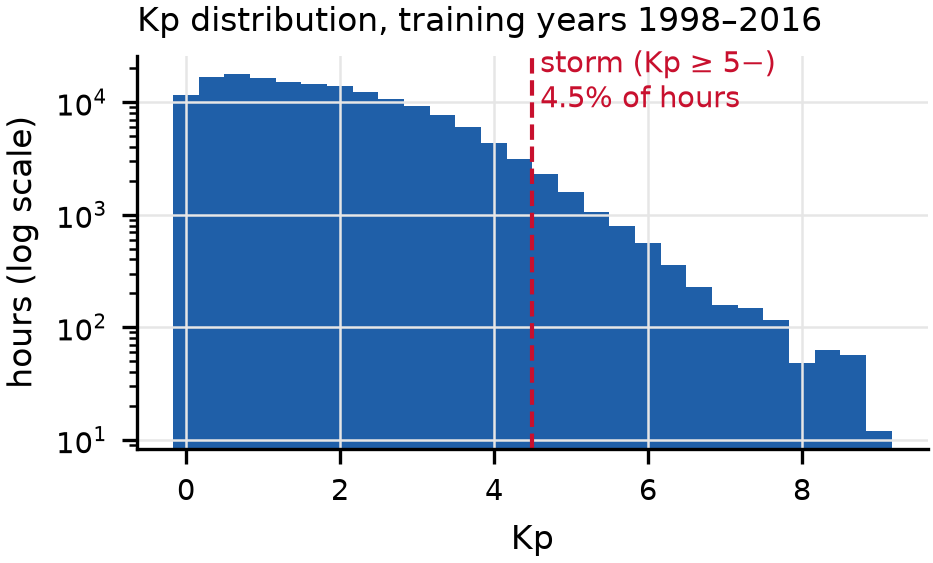
\includegraphics[width=\columnwidth]{eda1_kp_distribution.png}\\[3pt]
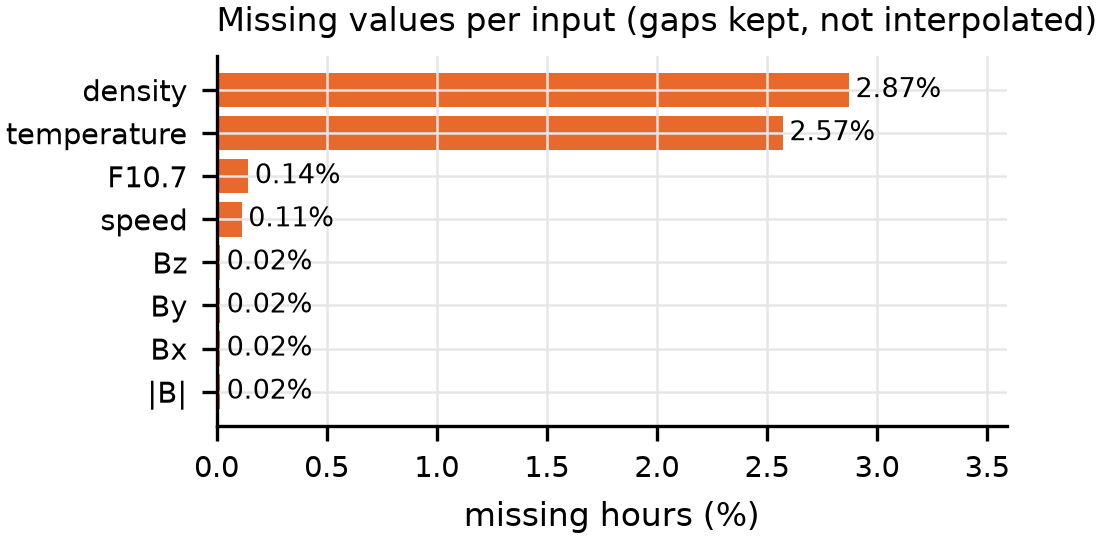
\includegraphics[width=\columnwidth]{eda2_missing.png}\\[3pt]
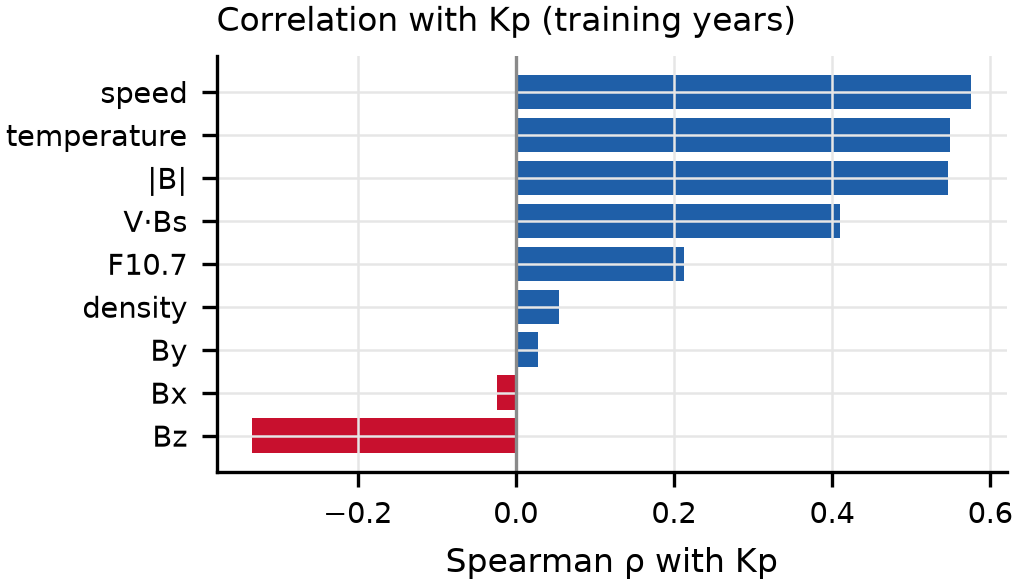
\includegraphics[width=\columnwidth]{eda3_correlation.png}
\caption{Class balance (top), missing values (middle) and Spearman correlation of each input with Kp (bottom).}\label{fig:eda1}
\end{figure}
\begin{figure}[t]\centering
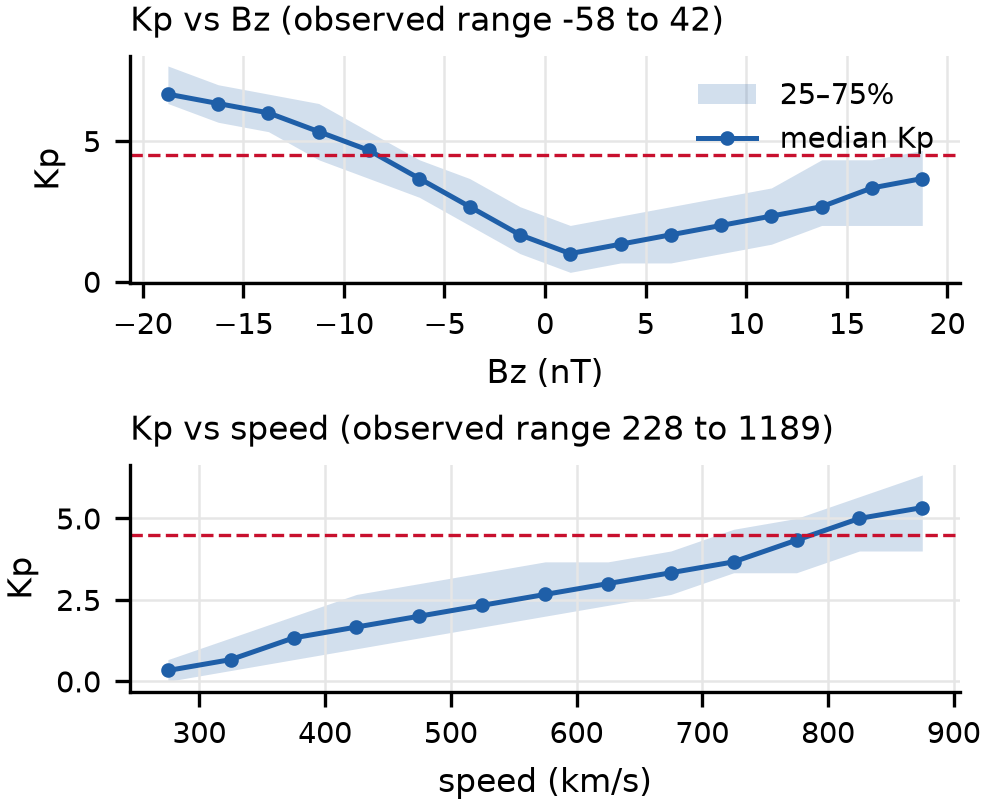
\includegraphics[width=\columnwidth]{eda4_kp_vs_drivers.png}\\[3pt]
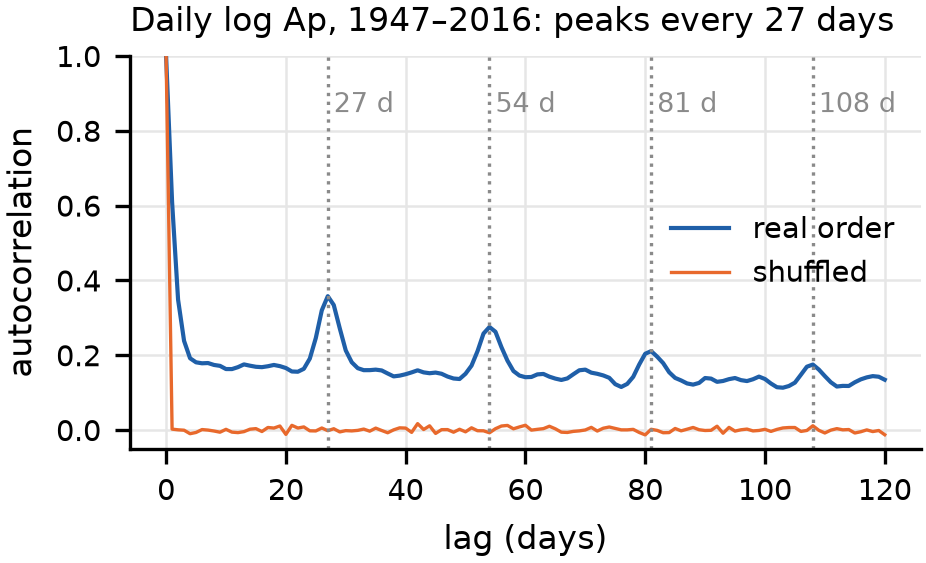
\includegraphics[width=\columnwidth]{eda5_ap_autocorrelation.png}
\caption{Median Kp and interquartile range against $B_z$ and speed (top two); autocorrelation of daily Ap with the
27-day echo (bottom).}\label{fig:eda2}
\end{figure}
\begin{figure}[t]\centering
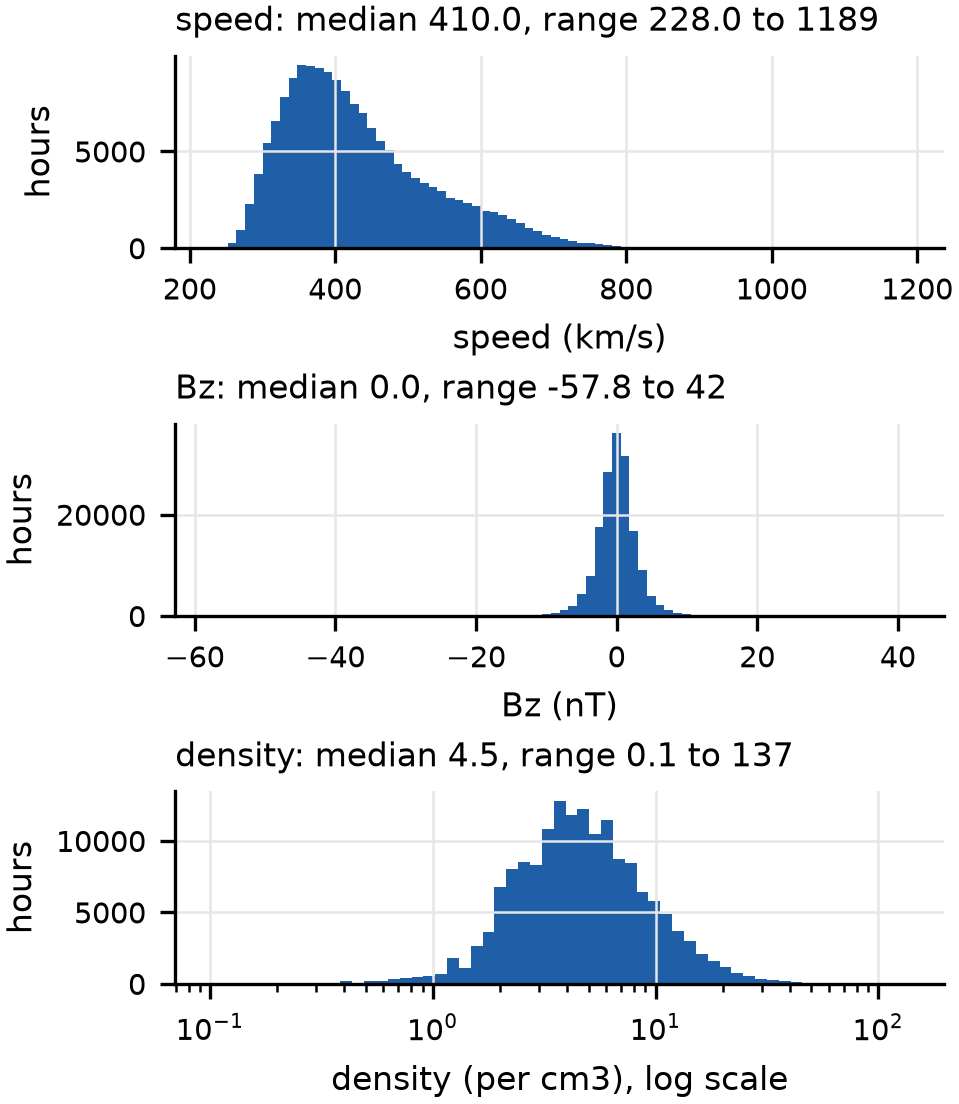
\includegraphics[width=\columnwidth]{eda6_input_distributions.png}
\caption{Distributions of speed, $B_z$ and density (training years); long tails are documented storms.}\label{fig:eda3}
\end{figure}

%=====================================================================================================================
\section{Methodology}
Figure~\ref{fig:pipe} traces the data from download to deployed model.

\begin{figure}[t]\centering
\begin{tikzpicture}[font=\scriptsize, node distance=1.8mm,
  b/.style={draw, rounded corners=1.5pt, align=left, text width=7.7cm, inner sep=3pt},
  ar/.style={-{Latex[length=1.4mm]}, thick}]
\node[b, fill=blue!6] (a) {\textbf{1. Ingest} by script: OMNI, GFZ, AIA images, NOAA (\code{src/download\_data.py})};
\node[b, fill=orange!10, below=of a] (b) {\textbf{2. Clean} (no fitted parameters): fill codes such as 9999 $\to$
missing; complete hourly grid with gaps kept; only definitive Kp as labels; F10.7 flare spikes ($>2\times$ the
27-day median) $\to$ missing};
\node[b, fill=orange!10, below=of b] (c) {\textbf{3. Label}: each hour gets its 3-hour block's Kp; each day $D$
gets targets for $D{+}1\ldots D{+}7$};
\node[b, fill=green!8, below=of c] (d) {\textbf{4. Features} (causal, shared by training and live use): 66 hourly
(nowcast); 29 index + 16 solar-wind + 7 coronal-hole daily (forecast)};
\node[b, fill=violet!8, below=of d] (e) {\textbf{5. Split} time-ordered: train / validation / test};
\node[b, fill=violet!8, below=of e] (f) {\textbf{6. Pipeline} fitted on training rows only: median imputation $\to$
standard scaling $\to$ model; \code{RandomizedSearchCV} over 5-fold \code{TimeSeriesSplit}};
\node[b, fill=violet!8, below=of f] (g) {\textbf{7. Evaluate} once on test; \textbf{save} with \code{joblib};
deploy; score every live forecast daily};
\foreach \i/\j in {a/b,b/c,c/d,d/e,e/f,f/g}{\draw[ar] (\i) -- (\j);}
\end{tikzpicture}
\caption{Pipeline from raw data to deployed model.}\label{fig:pipe}
\end{figure}

\subsection{Pre-processing and feature engineering}
\paragraph{Cleaning} Placeholder codes (e.g.\ 999.9, 9999) become missing. The data are put on a complete hourly
grid, so a 3-hour lag always means 3 hours even across gaps. F10.7 values more than twice their trailing 27-day
median are flare spikes, not the Sun's real activity level, and become missing.

\paragraph{Nowcaster features (66)} From 8 raw inputs: coupling functions ($-VB_z$, $VB_s$, Newell), dynamic
pressure, plasma $\beta$, Alfv\'en Mach number; lags of 1--9\,h; 3--24\,h windows (means, spread, extremes);
statistics since the current 3-hour block began; yesterday's F10.7 and its 81-day mean; and sin/cos of hour and day
of year. The sin/cos pair is the \textbf{encoding} of cyclic time (23:00 sits next to 00:00) and carries the
Russell--McPherron season effect \cite{russell1973}; there are no categorical inputs to one-hot encode.

\paragraph{Forecaster features (52)} 29 from past indices (Ap and max Kp of the last 7 days; 3/7/27-day means; Ap
27, 54 and 81 days before the target; F10.7; season), 16 from daily solar wind (issue day, day before, and the
27-day echo of speed), and 7 coronal-hole areas from the AIA image: pixels darker than $0.35\times$ the disk median
after a median filter, cleaned by a $7\times7$ morphological opening and a 300-pixel size filter
(Fig.~\ref{fig:ch}). Coronal holes emit fast wind that reaches Earth 2--4 days later \cite{vrsnak2007}.

\paragraph{Imputation and scaling} Median imputation and standard scaling sit inside a scikit-learn
\code{Pipeline} fitted on training rows only \cite{pedregosa2011}; they are needed by Linear Regression, KNN and
SVR. HistGB routes missing values natively.

\paragraph{Why feature engineering sits before the Pipeline} A \code{Pipeline} prevents leakage from steps that
\emph{learn} from data, by fitting them on training rows only. Our features learn nothing: each is a fixed formula
over the current and past hours, so it gives the same value inside or outside a \code{Pipeline} and cannot carry
test information. Every step that does learn is inside. Three reasons keep the features outside:
\begin{itemize}
\item \textbf{Lags need the continuous series.} A \code{Pipeline} sees only one fold's rows, so a 24-hour window or
81-day mean at the start of each fold would lose its history. We tested it: training features are identical, but
3.7\% of test rows and 7\% of each CV fold's rows change.
\item \textbf{Label rows are chosen after features}: only hours with definitive Kp are labels, but their lags come
from all hours, and a \code{Pipeline} cannot drop rows between steps.
\item \textbf{One module serves training and the live app}, so the two cannot compute features differently.
\end{itemize}

\subsection{Split, models and tuning}
\paragraph{Split (time-ordered, never shuffled)} Nowcaster: train 1998--2016 (166{,}560\,h, 68\%), validation
2017--2019 (26{,}280\,h, 11\%), test 2020--Jan 2026 (52{,}848\,h, 21\%). Forecaster: train from 1947; validation
2011--2019 year by year (each year forecast by a model trained on all earlier years); test 2020-01-01 to 2026-06-30
(2{,}373 days, 325 storm days).

\paragraph{Models} Nowcaster: persistence baseline (``Kp now = last block's Kp''), Linear Regression, KNN, SVR (RBF
kernel), Random Forest and HistGradientBoosting (HistGB) \cite{ke2017}. Forecaster: reference forecasts
(persistence, 27-day recurrence, 27-day mean, climatology), ARIMA/SARIMA/ARIMAX \cite{box2015}, LSTM, GRU, a
pretrained transformer used zero-shot, and HistGB with one model per lead day and target, so day-1 errors never
feed day 2. A HistGB classifier gives the storm-day probability.

\paragraph{Tuning} Each nowcaster model is tuned with \code{RandomizedSearchCV} over 5-fold \code{TimeSeriesSplit}
on the training years (every fold trains on the past and validates on the future). The forecaster uses the same
random search with 5 time-ordered folds and a 7-day \emph{gap}: a target lies up to 7 days after its issue day, so
without the gap the last training rows would carry targets inside the validation fold. Table~\ref{tab:params}
gives the final settings.

\begin{table}[h]\centering\footnotesize
\caption{Final model settings (scikit-learn \code{HistGradientBoosting*}, seed 42).}\label{tab:params}
\setlength{\tabcolsep}{3pt}
\begin{tabular}{@{}lcccc@{}}\toprule
 & Nowcast & Ap & max Kp & Storm\\\midrule
loss & squared & Poisson & Poisson & log loss\\
learning rate & 0.039 & 0.03 & 0.02 & 0.05\\
iterations & 700 & 200 & 400 & 300\\
max leaf nodes & 31 & 7 & 7 & 15\\
min samples / leaf & 50 & 200 & 400 & 100\\
L2 regularisation & 0.28 & 3.0 & 3.0 & 1.0\\\bottomrule
\end{tabular}
\end{table}

\paragraph{Prediction interval} Two quantile HistGB models (10th and 90th percentile) give an 80\% band, widened by
a conformalized-quantile-regression margin \cite{romano2019} estimated on out-of-fold training and validation years.

\paragraph{Adoption rules} Every change had to pass a rule written \emph{before} it ran, e.g.\ for the forecaster:
better pooled skill, better in at least 6 of 9 validation years, and storm skill not lower. Failed ideas (CME
catalogue, flare reports, intraday updates, log target) were rejected and kept on record.

\subsection{Leakage controls}
\begin{itemize}
\item \textbf{Causality tests:} features at time $t$ and forecasts for day $D$ must not change when every later row
is deleted (automated tests run on every push).
\item \textbf{Live = training:} a parity test shows identical features from the live and training code paths.
\item \textbf{Test never used for choices:} the validation code asserts it never reads 2020 or later; the final
model was committed to git before the test was run, and a marker file blocks a second run.
\item \textbf{Image control:} with the solar images moved to random dates the coronal-hole gain disappears, so it
comes from real images on their real dates.
\end{itemize}
All test scores come from models fitted only on data up to 2019. After scoring, the deployed models were refitted
on all data up to 2026, so from then on their evidence is the live log.

\begin{figure}[t]\centering
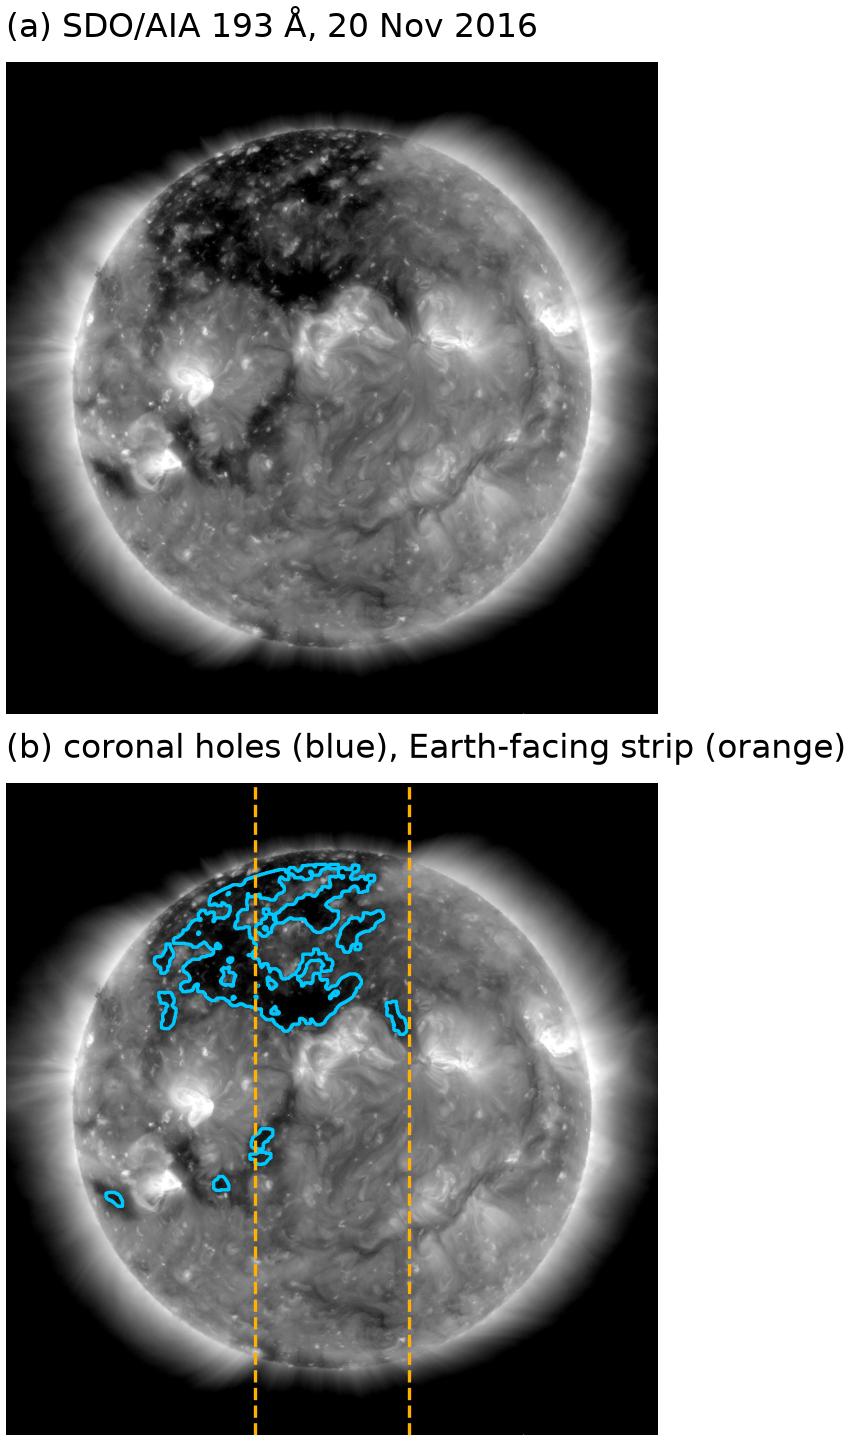
\includegraphics[width=0.78\columnwidth]{res_coronal_hole.png}
\caption{Coronal-hole detection on one AIA 193\,\AA{} image: (a) the image; (b) detected holes and the
Earth-facing strip used as a forecaster input.}\label{fig:ch}
\end{figure}

%=====================================================================================================================
\section{Results}
\subsection{Nowcaster}
\begin{table}[h]\centering\footnotesize
\caption{Nowcaster RMSE (Kp) on every split. Storm = test hours with Kp\,$\ge$\,5$-$. Test 2020--Jan 2026, 52{,}848 hours.}\label{tab:now}
\setlength{\tabcolsep}{3pt}
\begin{tabular}{@{}lcccccc@{}}\toprule
Model & Train & CV & Val & Test & Test $R^2$ & Storm\\\midrule
Persistence & -- & -- & 0.819 & 0.862 & 0.566 & 1.368\\
Linear Reg. & 0.689 & 0.665 & 0.595 & 0.665 & 0.742 & 1.470\\
KNN & 0.000 & 0.696 & 0.614 & 0.657 & 0.748 & 1.337\\
SVR & 0.541 & 0.618 & 0.557 & 0.605 & 0.786 & 1.079\\
Random Forest & 0.545 & 0.644 & 0.564 & 0.606 & 0.785 & 0.972\\
\textbf{HistGB} & 0.534 & \textbf{0.561} & \textbf{0.522} & \textbf{0.573} & \textbf{0.808} & \textbf{0.846}\\\bottomrule
\end{tabular}
\end{table}

HistGB is the best model on every split (Table~\ref{tab:now}, Fig.~\ref{fig:models}): 34\% below persistence
overall and 38\% on storm hours.

\paragraph{Over- and under-fitting} HistGB's train, CV and validation RMSE are close (0.534 / 0.561 / 0.522), so
it does not overfit. KNN memorises the training data (train RMSE $\approx$\,0, validation 0.614), and Linear
Regression underfits (train error 0.689 above its validation error). The learning curve (Fig.~\ref{fig:fit}a)
shows the train--validation gap closing with more data, and doubling the data gains only 0.003. In the complexity
curve (Fig.~\ref{fig:fit}b) validation RMSE is flat from 31 to 127 leaves while train RMSE keeps falling, so larger
trees only memorise. The remaining error is an information limit of single-point L1 measurements, not a lack of
model capacity.

\paragraph{Errors} Error grows with storm level (Fig.~\ref{fig:level}) and large storms are under-predicted
(G3+ bias $-$0.57 Kp for HistGB, $-$0.93 for persistence): rare extremes are pulled towards the mean. Onsets appear
1--2\,h late, because a 3-hour block's driver has not fully arrived in its first hour. The May 2024 G5 storm, never
seen in training, is tracked from onset to recovery with a predicted peak of 8.6 against an observed 9
(Fig.~\ref{fig:may}). The 80\% interval covers 80.8\% of test hours (75.7\% before the conformal correction).

\begin{figure}[t]\centering
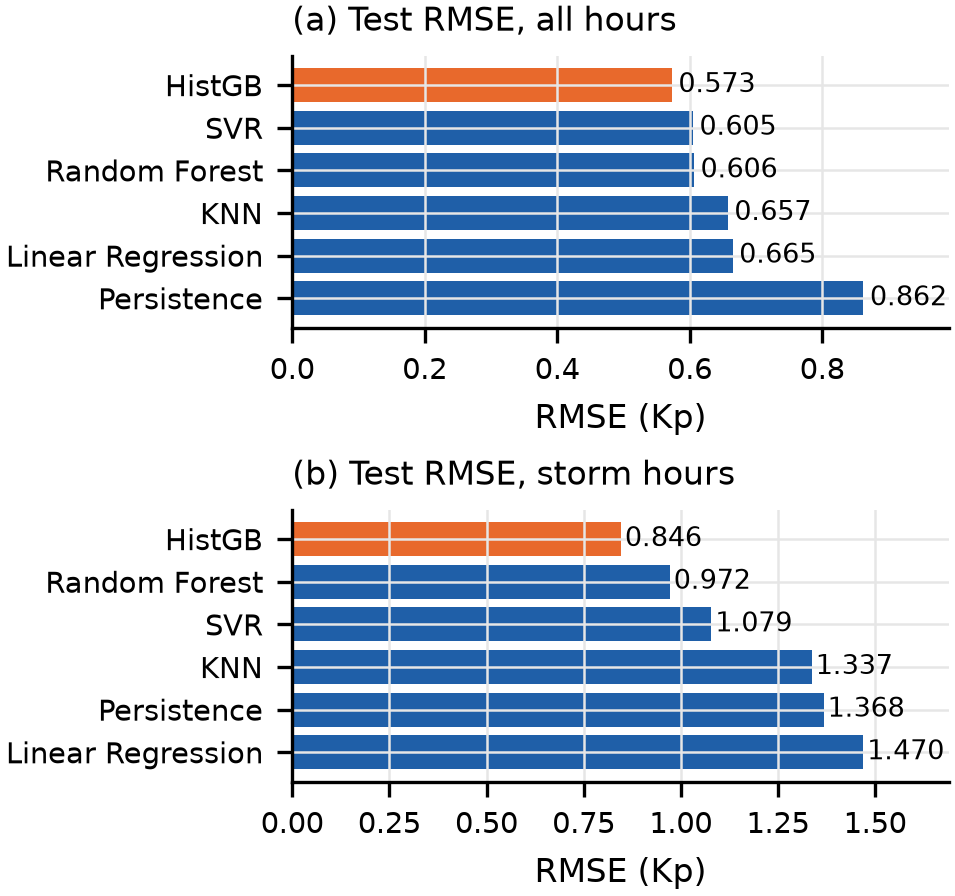
\includegraphics[width=\columnwidth]{res_model_comparison.png}
\caption{Nowcaster test RMSE per model: (a) all hours; (b) storm hours.}\label{fig:models}
\end{figure}
\begin{figure}[t]\centering
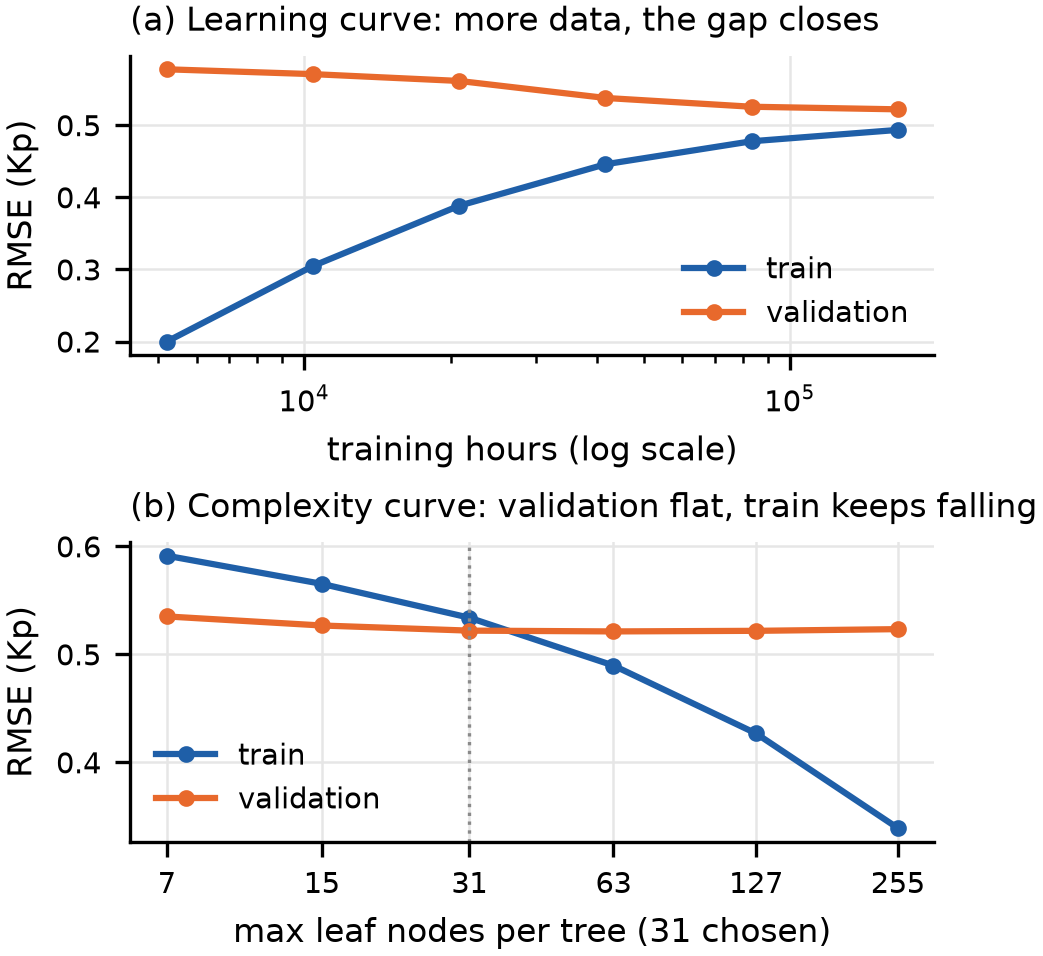
\includegraphics[width=\columnwidth]{res_fitting_curves.png}
\caption{Nowcaster (a) learning curve and (b) complexity curve: train vs validation RMSE.}\label{fig:fit}
\end{figure}
\begin{figure}[t]\centering
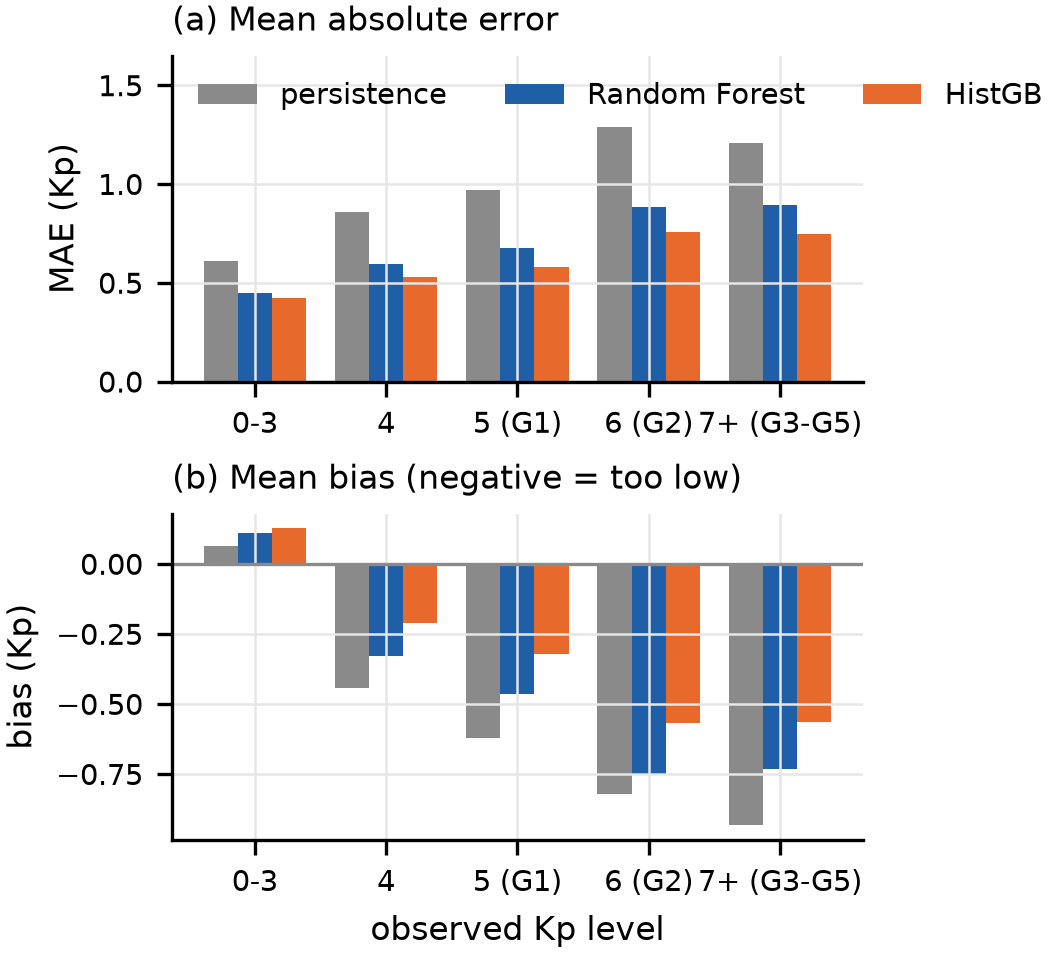
\includegraphics[width=\columnwidth]{res_error_by_level.png}
\caption{Test error by observed storm level: (a) mean absolute error; (b) mean bias.}\label{fig:level}
\end{figure}
\begin{figure}[t]\centering
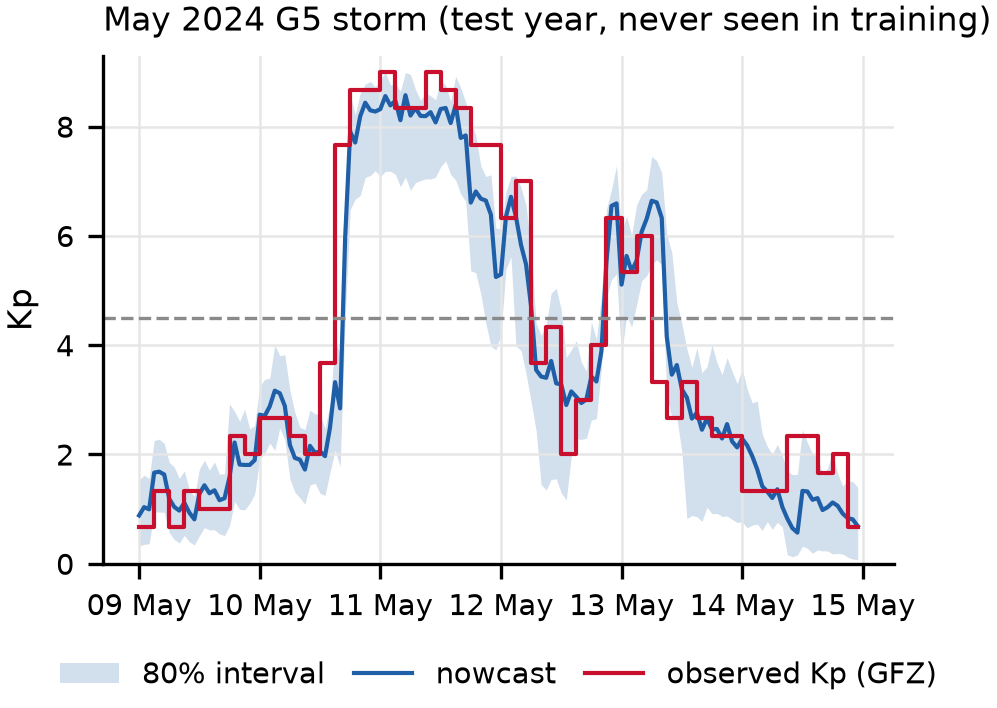
\includegraphics[width=\columnwidth]{res_may2024.png}
\caption{Nowcast of the May 2024 G5 storm with its 80\% interval (test year).}\label{fig:may}
\end{figure}

\subsection{Forecaster}
\begin{table}[h]\centering\footnotesize
\caption{Forecaster, test 2020-01 to 2026-06: daily Ap RMSE by lead day and skill against the 27-day mean
(1 = perfect, 0 = no better than the 27-day mean).}\label{tab:fc}
\setlength{\tabcolsep}{3pt}
\begin{tabular}{@{}lccccc@{}}\toprule
Model & day 1 & day 2 & day 3 & day 7 & skill\\\midrule
\textbf{Final model} & \textbf{10.67} & 11.80 & \textbf{11.73} & \textbf{11.95} & \textbf{0.122}\\
HistGB (indices only) & 10.78 & 11.98 & 11.91 & 12.01 & 0.100\\
NOAA official & 10.89 & \textbf{11.73} & 11.90 & -- & --\\
ARIMAX & 10.96 & -- & 12.15 & 12.17 & 0.069\\
Pretrained transformer & 11.83 & -- & 12.66 & 12.65 & $-$0.015\\
27-day mean & 12.27 & 12.42 & 12.45 & 12.48 & 0\\\bottomrule
\end{tabular}
\end{table}
\begin{table}[h]\centering\footnotesize
\caption{Storm warnings of the final model on the test period (325 storm days).}\label{tab:storm}
\setlength{\tabcolsep}{4pt}
\begin{tabular}{@{}lccccc@{}}\toprule
Day & Heidke & Detected & False al. & F1 & Indices only\\\midrule
1 & \textbf{0.40} & 53\% & 54\% & 0.49 & 0.34\\
2 & \textbf{0.26} & 40\% & 65\% & 0.37 & 0.20\\
3 & \textbf{0.25} & 30\% & 61\% & 0.34 & 0.20\\
4 & \textbf{0.22} & 29\% & 65\% & 0.32 & 0.21\\
5 & 0.21 & 36\% & 70\% & 0.33 & \textbf{0.22}\\
6 & \textbf{0.21} & 54\% & 74\% & 0.35 & 0.20\\
7 & \textbf{0.22} & 34\% & 68\% & 0.33 & 0.19\\\bottomrule
\end{tabular}
\end{table}

\paragraph{Values} The final model beats the index-only HistGB at every lead day (Table~\ref{tab:fc},
Fig.~\ref{fig:fc}a). A Diebold--Mariano test \cite{diebold1995} on daily squared errors finds the gain significant on
days 2--5 ($p\le0.025$), exactly the 2--4 day travel time of fast wind from a coronal hole. The 95\% block-bootstrap
interval of the skill gain is $+0.007$ to $+0.050$, so it is not chance. Against NOAA's official forecast it is ahead
on days 1 and 3 and behind on day 2, with no significant difference ($p$ = 0.69 / 0.91 / 0.55).

\paragraph{Storm warnings} Classification metrics are in Table~\ref{tab:storm} and Fig.~\ref{fig:conf}. On day 1
the model catches 53\% of storm days with 54\% of its warnings false (F1 0.49). Heidke skill (0 = chance,
1 = perfect) is clearly better than the index-only model on days 1--3, with fewer false alarms, and about equal on
days 4--7. Skill falls with lead time (F1 0.32--0.37 from day 2) because storms caused by sudden solar eruptions
cannot be seen days ahead; on day 6 a lower warning threshold catches more storms at the cost of more false
alarms.

\begin{figure}[t]\centering
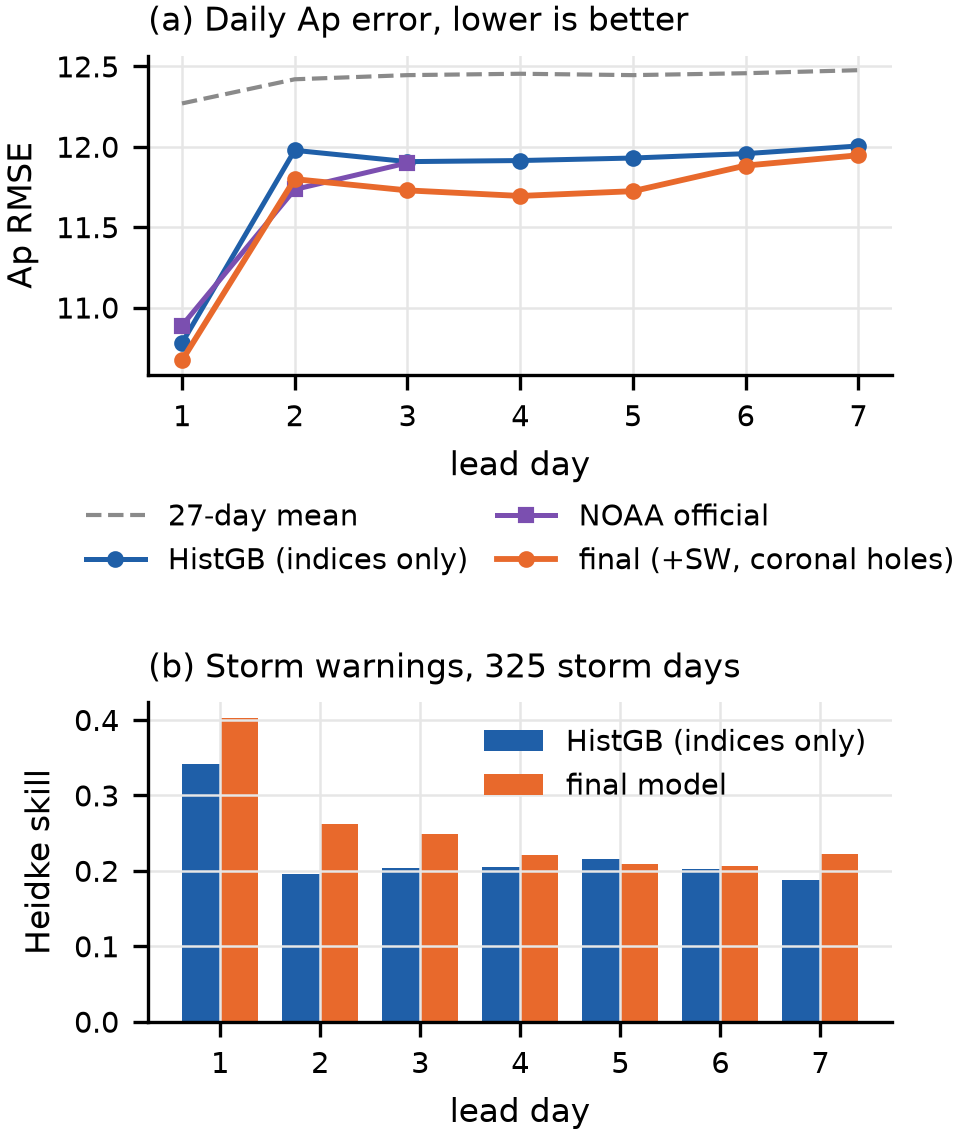
\includegraphics[width=\columnwidth]{res_forecaster_test.png}
\caption{Forecaster test: (a) daily Ap error by lead day; (b) storm-warning Heidke skill.}\label{fig:fc}
\end{figure}
\begin{figure}[t]\centering
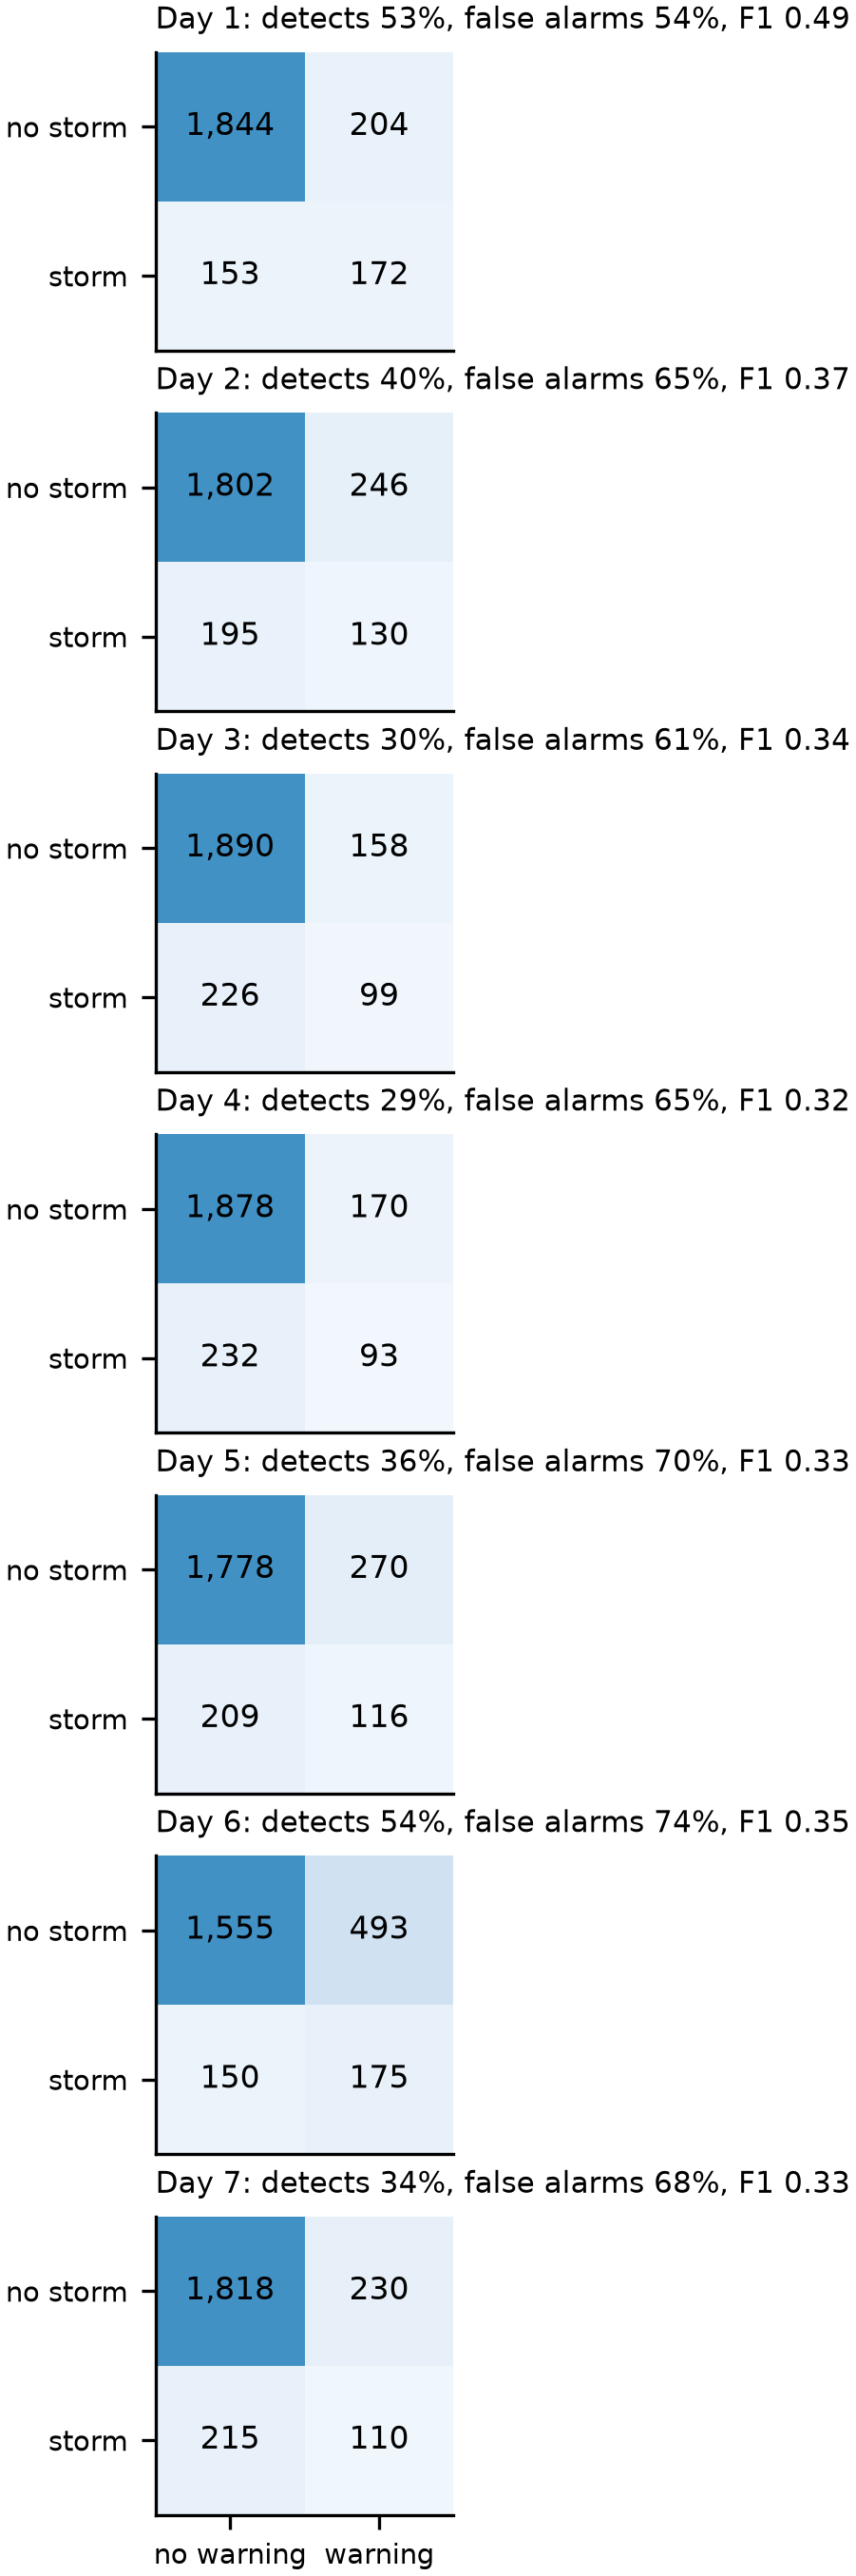
\includegraphics[width=0.85\columnwidth]{res_storm_confusion.png}
\caption{Confusion matrices of the final model's storm warnings on the test period, lead days 1--7 (2{,}373 days,
325 storm days).}\label{fig:conf}
\end{figure}

%=====================================================================================================================
\section{Deployment}
The project is deployed on \textbf{all three platforms} required by the course. All three load the same
\code{joblib} model files and call the same prediction code; package versions are pinned in \code{requirements.txt}.
\begin{enumerate}
\item \textbf{Streamlit Community Cloud}, \url{https://tormenta.streamlit.app/} (Figs.~\ref{fig:app1}--\ref{fig:app2}).
Six pages: Overview, Forecast, Explore (replay any past day), Scorecard, Nowcast and Method. It has an input form
(the what-if explorer), predictions with an 80\% range and a storm probability, explanatory charts, and live data
refreshed every few minutes.
\item \textbf{Hugging Face Hub}: the model, pipeline code and model card at
\url{https://huggingface.co/aliza-ayaz/tormenta}, and a live Space running the same Streamlit app in the browser at
\url{https://huggingface.co/spaces/aliza-ayaz/tormenta}.
\item \textbf{Local Flask app}: \code{python app/flask\_app/app.py} serves \url{http://127.0.0.1:5000} with an HTML
form, a \code{/predict} endpoint (form or JSON), \code{/api/forecast}, and per-field input validation with clear
error messages (e.g.\ ``speed must be a number'').
\end{enumerate}
\textbf{Automation.} A daily GitHub Actions job issues the 7-day forecast, saves NOAA's forecasts, scores every
forecast whose day has arrived, and commits append-only logs; forecasts are never edited. A weekly check retrains
only after two degraded health checks and promotes a model only if it beats the current one on unseen data. The
final model of this report runs in \emph{shadow mode} (issued and logged every day, but not shown) for three
weeks before it replaces the live forecaster.

\begin{figure}[t]\centering
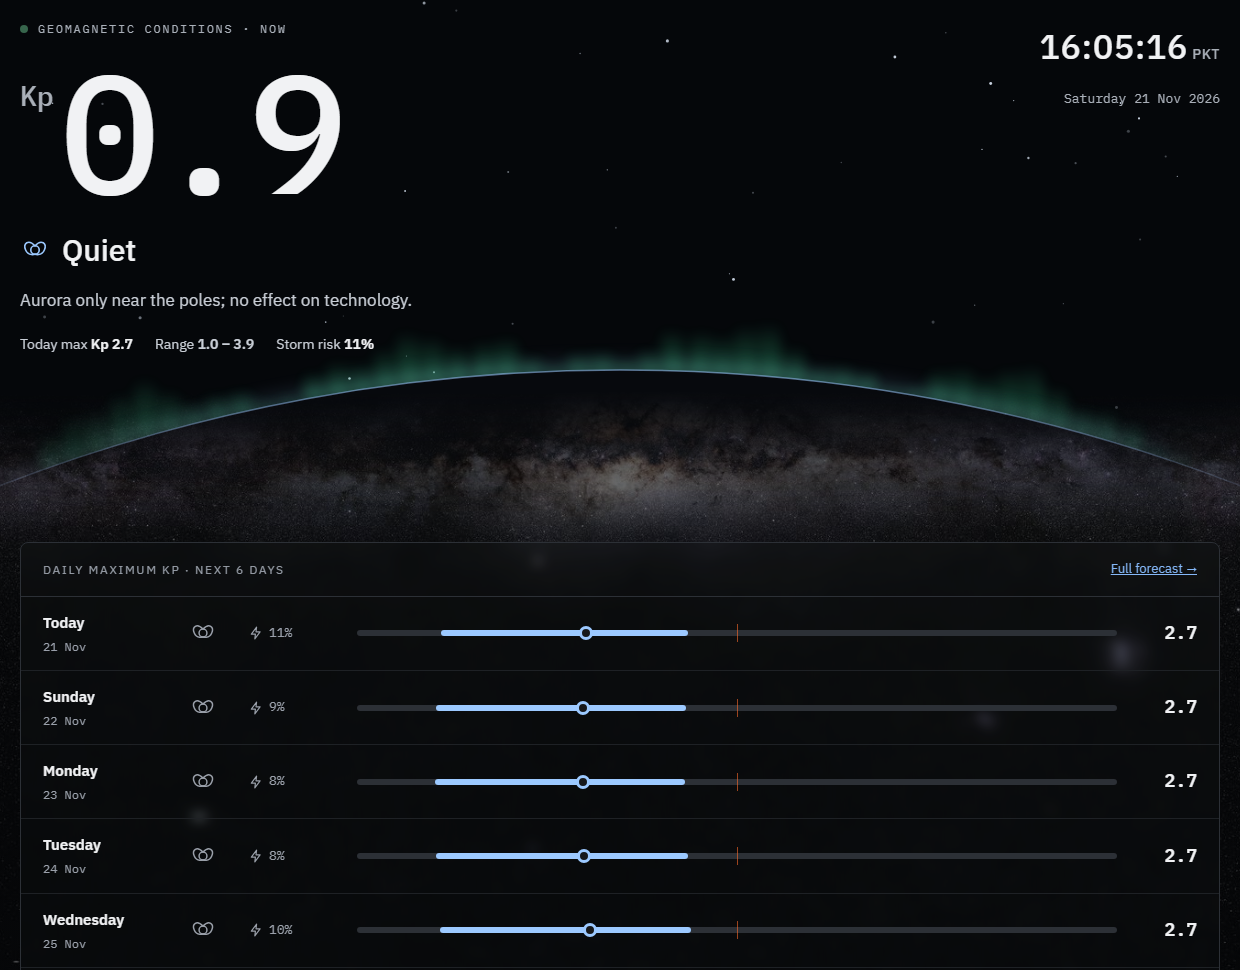
\includegraphics[width=\columnwidth]{app_dark_overview.png}\\[3pt]
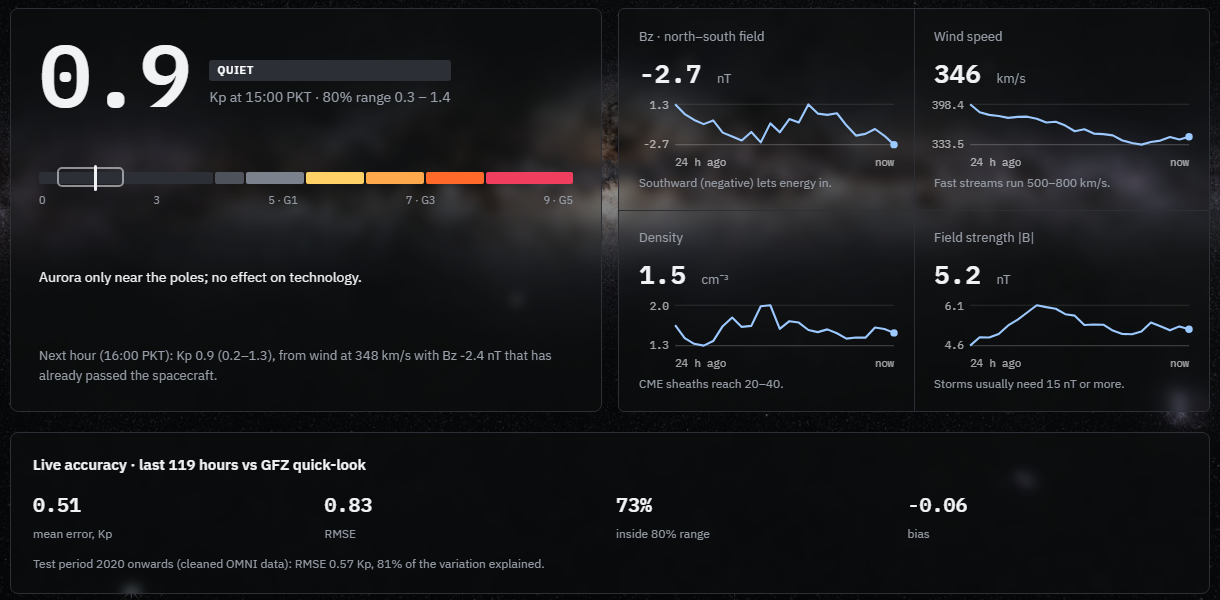
\includegraphics[width=\columnwidth]{app_dark_nowcast.png}
\caption{Streamlit app (dark theme): Overview with Kp now and the next six days (top); Nowcast with Kp, its 80\%
range and the live solar wind (bottom).}\label{fig:app1}
\end{figure}
\begin{figure}[t]\centering
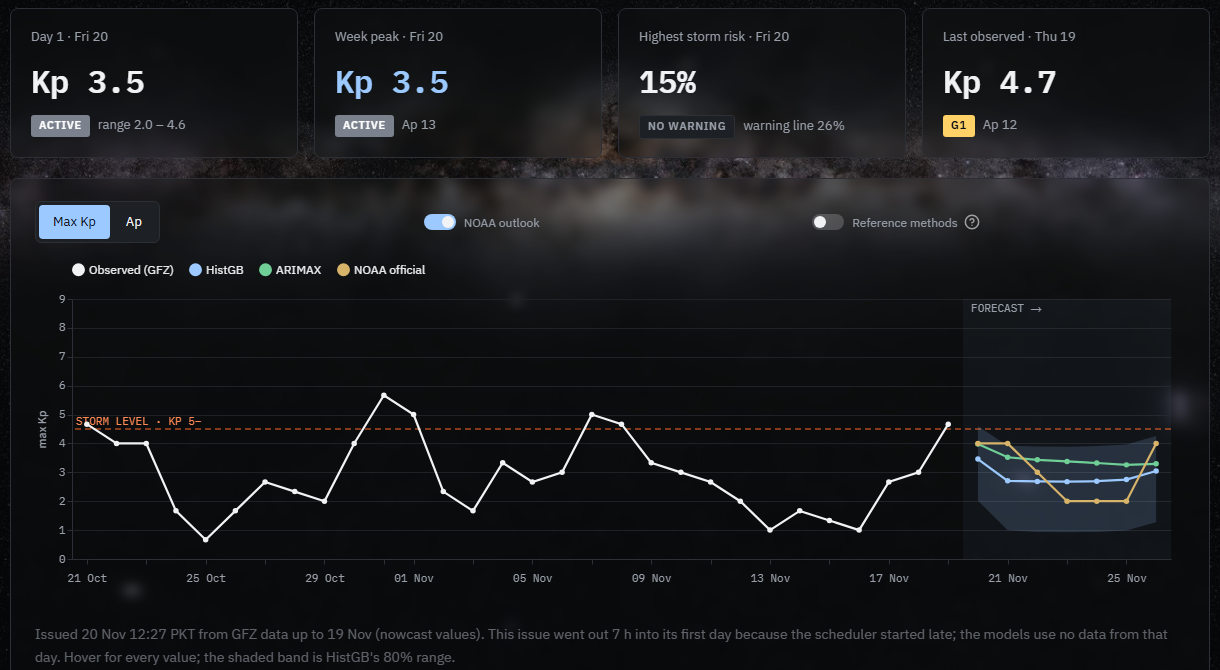
\includegraphics[width=\columnwidth]{app_dark_forecast.png}
\caption{Streamlit app (dark theme): 7-day forecast with storm risk, NOAA's official outlook and the 80\% range.}\label{fig:app2}
\end{figure}

%=====================================================================================================================
\FloatBarrier
\section{Limitations and future work}
\begin{itemize}
\item \textbf{Sudden eruptions.} Storms from coronal mass ejections are invisible in our inputs until they arrive,
so the first storm day is usually missed: both the live and the final model missed the onset of the May 2024 storm
on 10 May and warned for the next three storm days.
\item \textbf{Extremes.} Kp\,9 is very rare in training, so storm size is under-predicted and trees cannot
extrapolate beyond the largest values seen; during storms the storm warning is the number to trust.
\item \textbf{Lead time.} The nowcast sees at most about one hour ahead, the solar wind's travel time from L1.
\item \textbf{Quiet validation years.} 2017--2019 is a solar minimum; the comparison of storm warnings with NOAA
rests on 91 storm days.
\item \textbf{Live inputs.} Real-time data are noisier than the corrected archives used for training; the final
forecaster's shadow run checks this before it goes live.
\end{itemize}
\textbf{Future work:} detecting eruptions from coronagraph images, sub-hourly solar-wind variability, probabilistic
Kp forecasts 1--3 hours ahead, and a journal paper on the coronal-hole forecaster.

%=====================================================================================================================
\balance
\begin{thebibliography}{13}
\bibitem{matzka2021} J.~Matzka, C.~Stolle, Y.~Yamazaki, O.~Bronkalla, and A.~Morschhauser, ``The geomagnetic Kp index and derived indices of geomagnetic activity,'' \emph{Space Weather}, vol.~19, Art.~no.~e2020SW002641, 2021.
\bibitem{gfzkp} J.~Matzka, O.~Bronkalla, K.~Tornow, K.~Elger, and C.~Stolle, ``Geomagnetic Kp index,'' V.~1.0, GFZ Data Services, 2021, doi: 10.5880/Kp.0001.
\bibitem{king2005} J.~H. King and N.~E. Papitashvili, ``Solar wind spatial scales in and comparisons of hourly Wind and ACE plasma and magnetic field data,'' \emph{J. Geophys. Res.}, vol.~110, Art.~no.~A02104, 2005.
\bibitem{lemen2012} J.~R. Lemen \emph{et al.}, ``The Atmospheric Imaging Assembly (AIA) on the Solar Dynamics Observatory (SDO),'' \emph{Sol. Phys.}, vol.~275, pp.~17--40, 2012.
\bibitem{swpc} NOAA Space Weather Prediction Center, ``Real-time solar wind and forecast products.'' [Online]. Available: \url{https://www.swpc.noaa.gov}
\bibitem{newell2007} P.~T. Newell, T.~Sotirelis, K.~Liou, C.-I. Meng, and F.~J. Rich, ``A nearly universal solar wind-magnetosphere coupling function inferred from 10 magnetospheric state variables,'' \emph{J. Geophys. Res.}, vol.~112, Art.~no.~A01206, 2007.
\bibitem{russell1973} C.~T. Russell and R.~L. McPherron, ``Semiannual variation of geomagnetic activity,'' \emph{J. Geophys. Res.}, vol.~78, no.~1, pp.~92--108, 1973.
\bibitem{vrsnak2007} B.~Vr\v{s}nak, M.~Temmer, and A.~M. Veronig, ``Coronal holes and solar wind high-speed streams: II. Forecasting the geomagnetic effects,'' \emph{Sol. Phys.}, vol.~240, pp.~331--346, 2007.
\bibitem{pedregosa2011} F.~Pedregosa \emph{et al.}, ``Scikit-learn: Machine learning in Python,'' \emph{J. Mach. Learn. Res.}, vol.~12, pp.~2825--2830, 2011.
\bibitem{ke2017} G.~Ke \emph{et al.}, ``LightGBM: A highly efficient gradient boosting decision tree,'' in \emph{Proc. Adv. Neural Inf. Process. Syst. (NeurIPS)}, 2017.
\bibitem{box2015} G.~E.~P. Box, G.~M. Jenkins, G.~C. Reinsel, and G.~M. Ljung, \emph{Time Series Analysis: Forecasting and Control}, 5th~ed. Hoboken, NJ, USA: Wiley, 2015.
\bibitem{romano2019} Y.~Romano, E.~Patterson, and E.~Cand\`es, ``Conformalized quantile regression,'' in \emph{Proc. Adv. Neural Inf. Process. Syst. (NeurIPS)}, 2019.
\bibitem{diebold1995} F.~X. Diebold and R.~S. Mariano, ``Comparing predictive accuracy,'' \emph{J. Bus. Econ. Stat.}, vol.~13, no.~3, pp.~253--263, 1995.
\end{thebibliography}

%=====================================================================================================================
\section*{Individual Contributions}
Syeda Aliza Ayaz and Husn ur Rehman worked jointly on every stage and contributed equally; each wrote and reviewed
code in every area, so both can explain every part.

\vspace{4pt}
\noindent{\centering\footnotesize
\begin{tabular}{@{}p{1.7cm}p{5.0cm}p{0.7cm}@{}}\toprule
Stage & Work & By\\\midrule
Problem & topic, targets, success metrics, proposal & Both\\
Data & OMNI, GFZ, AIA, NOAA ingestion; cleaning; download script & Both\\
EDA & 15 plots and their findings & Both\\
Features & 66 nowcast and 52 forecast features; coronal-hole detection & Both\\
Modelling & baselines, nowcast and forecast models, tuning, intervals & Both\\
Evaluation & validation, one-time tests, NOAA comparison, leakage tests & Both\\
Deployment & Streamlit, Hugging Face, Flask, daily automation & Both\\
Report & writing, figures, demo and viva preparation & Both\\\bottomrule
\end{tabular}\par}

\end{document}
